
\section{Introduction}
Impedance spectroscopy, introduced in \cpageref{characterization_impedance}, is a powerful technique for characterizing electronic devices in the frequency domain.
The first information that can be directly extracted from impedance spectroscopy is a frequency\hyp{}dependent capacitance \cite{Brus2016}.
When studying this in perovskite solar cells, the results are of difficult interpretation \cite{Almora2018,Guillen2014}.
A giant capacitance is always observed at low frequencies for illuminated devices \cite{Juarez-Perez2014,Kim2015c}.
More rarely, also a negative capacitance (\textsl{i.e.} an inductance) has been observed in perovskite solar cell \cite{Ghahremanirad2017,Guerrero2016,Sanchez2014} and other kinds of solar cells \cite{Mora-Sero2006,Knapp2015}.
In order to extract the individual parameters, like transport and recombination constants, the data has to be fitted using an electronic equivalent circuit \cite{Jamnik2001}.
The components of the circuit should have a relation with the actually existing processes, so that we can relate the parameters of the electrical component with the solar cell specific internal mechanisms.
Many complex circuits have been proposed in literature, some of them included inductors for matching the inductive behaviour \cite{Almora2018,Ghahremanirad2017,Guerrero2016}.
Previously to our publication, these phenomena were interpreted as caused by a huge free charge accumulation at the interfaces due to the influence of ionic accumulation \cite{Guerrero2016,Zarazua2016a} supported by drift\hyp{}diffusion simulations \cite{Garcia-Rosell2018,Lopez-Varo2018}.
It has to be noted that any slow process causing a change in the flowing current could result in an apparent capacitance or inductance, this could happen with degradation processes or heating \cite{Knapp2015}.
In perovskite solar cells, the electrostatic potential arising from mobile ion redistribution controls electronic charge transfer barriers \cite{Tress2016,Pockett2017}.
In May 2018 we uploaded to ArXiv a pre-print which was then published in \authoryear{Moia2019} with an alternative interpretation for the giant capacitance: this influence of the ionic charge on the electronic processes such as recombination and can give rise to apparent capacitive behaviour.
This effect does not involve an accumulation of an enormous amount of charge, as it was expected by a giant capacitance, so it cannot be described by a capacitor in the equivalent electrical circuit.
For the inductive behaviour we proposed that the same influence can affect the charge injection causing a negative apparent capacitance.
More or less at the same time, other research groups published similar interpretations \cite{Ebadi2019,Jacobs2018}.
We proposed that both of the effects (apparent capacitance and inductance) can be described by transistors element in the circuit.
This allows the charge to flow through an interface to not only depend on the applied voltage, like in a common diode, but also on an external influence: the ionic density close to the interface.
The influence of ionic migration on electronic transfer can be thought as an amplification of electronic current by ionic current.
Our model not only works in the small perturbation regime employed in impedance spectroscopy, but can also explain data from hysteretic current\hyp{}voltage sweeps.
The understanding of this mechanism not only allows the researcher to successfully use impedance spectroscopy on perovskite solar cells and other ionic and electronic interfaces (e.g. electrochemical communication between neurons in the brain \cite{Cole1956}) but could also be employed for designing new physical electronic components showing large and tunable apparent capacitance or inductance in a reduced volume.

\paragraph{Design of the Experiment}
Impedance spectroscopy has been initially modelled studying the current evolution after a single voltage step.
This first rough attempt should be polished using Kramers\hyp{}Kronig relation and has not been published yet.
In order to confirm the initial observations, the impedance spectroscopy has been implemented trying to match the actual experimental conditions.
For this reason, the oscillating current obtained when applying an oscillating voltage has been studied separately for each frequency.
This caused the simulation to be much slower but still doable with my laptop.
Additionally, the phase and amplitude has been obtained mimicking the demodulation of a lock-in amplifier rather than with a sinusoidal fitting.

\paragraph{Author contributions}
I implemented and run the impedance spectroscopy simulation on top of Driftfusion software developed by Dr.\ Phil Calado, Dr.\ Piers RF Barnes, Mohammed Azzouzi, Benjamin Hilton, and myself.
Dr.\ Davide Moia and Dr.\ Piers RF Barnes created the formalism and the electrical equivalent circuit.
William Fisher and Dr. Davide Moia fitted the experimental data using fitting routines developed by Dr.\ Piers RF Barnes.
Dr.\ Michael Stringer, Dr.\ Onkar Game, Yinghong Hu, Dr.\ David Lidzey, and Dr.\ Pablo Docampo provided excellently stable perovskite solar cells to be studied.


\section{Implementation}

	fromISwaveEAStructToTxt.m
fromISwaveResultsToTxt.m
IS_full_analysis_impedance.m
ISwave_EA_single_demodulation.m
ISwave_EA_single_exec.m
ISwave_EA_single_fit.m
ISwave_full_analysis_nyquist.m
ISwave_full_analysis_phase.m
ISwave_full_exec.m
ISwave_full_exec_nonparallel.m
ISwave_single_analysis.m
ISwave_subtracting_analysis.m


\section{Measured and simulated impedance spectra characteristics}

	\subsection{Calculation of Ionic Displacement Current}\label{displacement_current_ionic}
		As seen in \cpageref{intro_displacement_current}

\subsection{Apparent Capacitance of a Device in Dark}
\paragraph{High frequency}
\paragraph{Mid frequency}
\paragraph{Low frequency}
The ionic influence on the dark capacitance has already been reported by \authoryear{Yang2015e}.

\subsection{Apparent Capacitance of an Illuminated Device}
\paragraph{High frequency}
\paragraph{Mid frequency}
\paragraph{Low frequency}

%\section{Ionic-to-electronic current amplification}
%\section{Capacitor-like and inductor-like behaviour}


\subsection{Large perturbations}\label{impedance-large_perturbations}
A too wide sinusoidal voltage oscillation amplitude in impedance measurements can cause a non-sinusoidal current output.
This is not a problem for the measurement itself, as the lock-in amplifiers are perfectly able to extract the amplitude and the phase of the signal first harmonic, ignoring the higher harmonics caused by the too large perturbation.
But artefacts could arise and cause misinterpretations.



\section{Further development}


\begin{figure}
	\makebox[\textwidth][c]{
		\parbox{1.1\textwidth}{
			\centering
			\begin{subfigure}[t]{0.51\textwidth}
				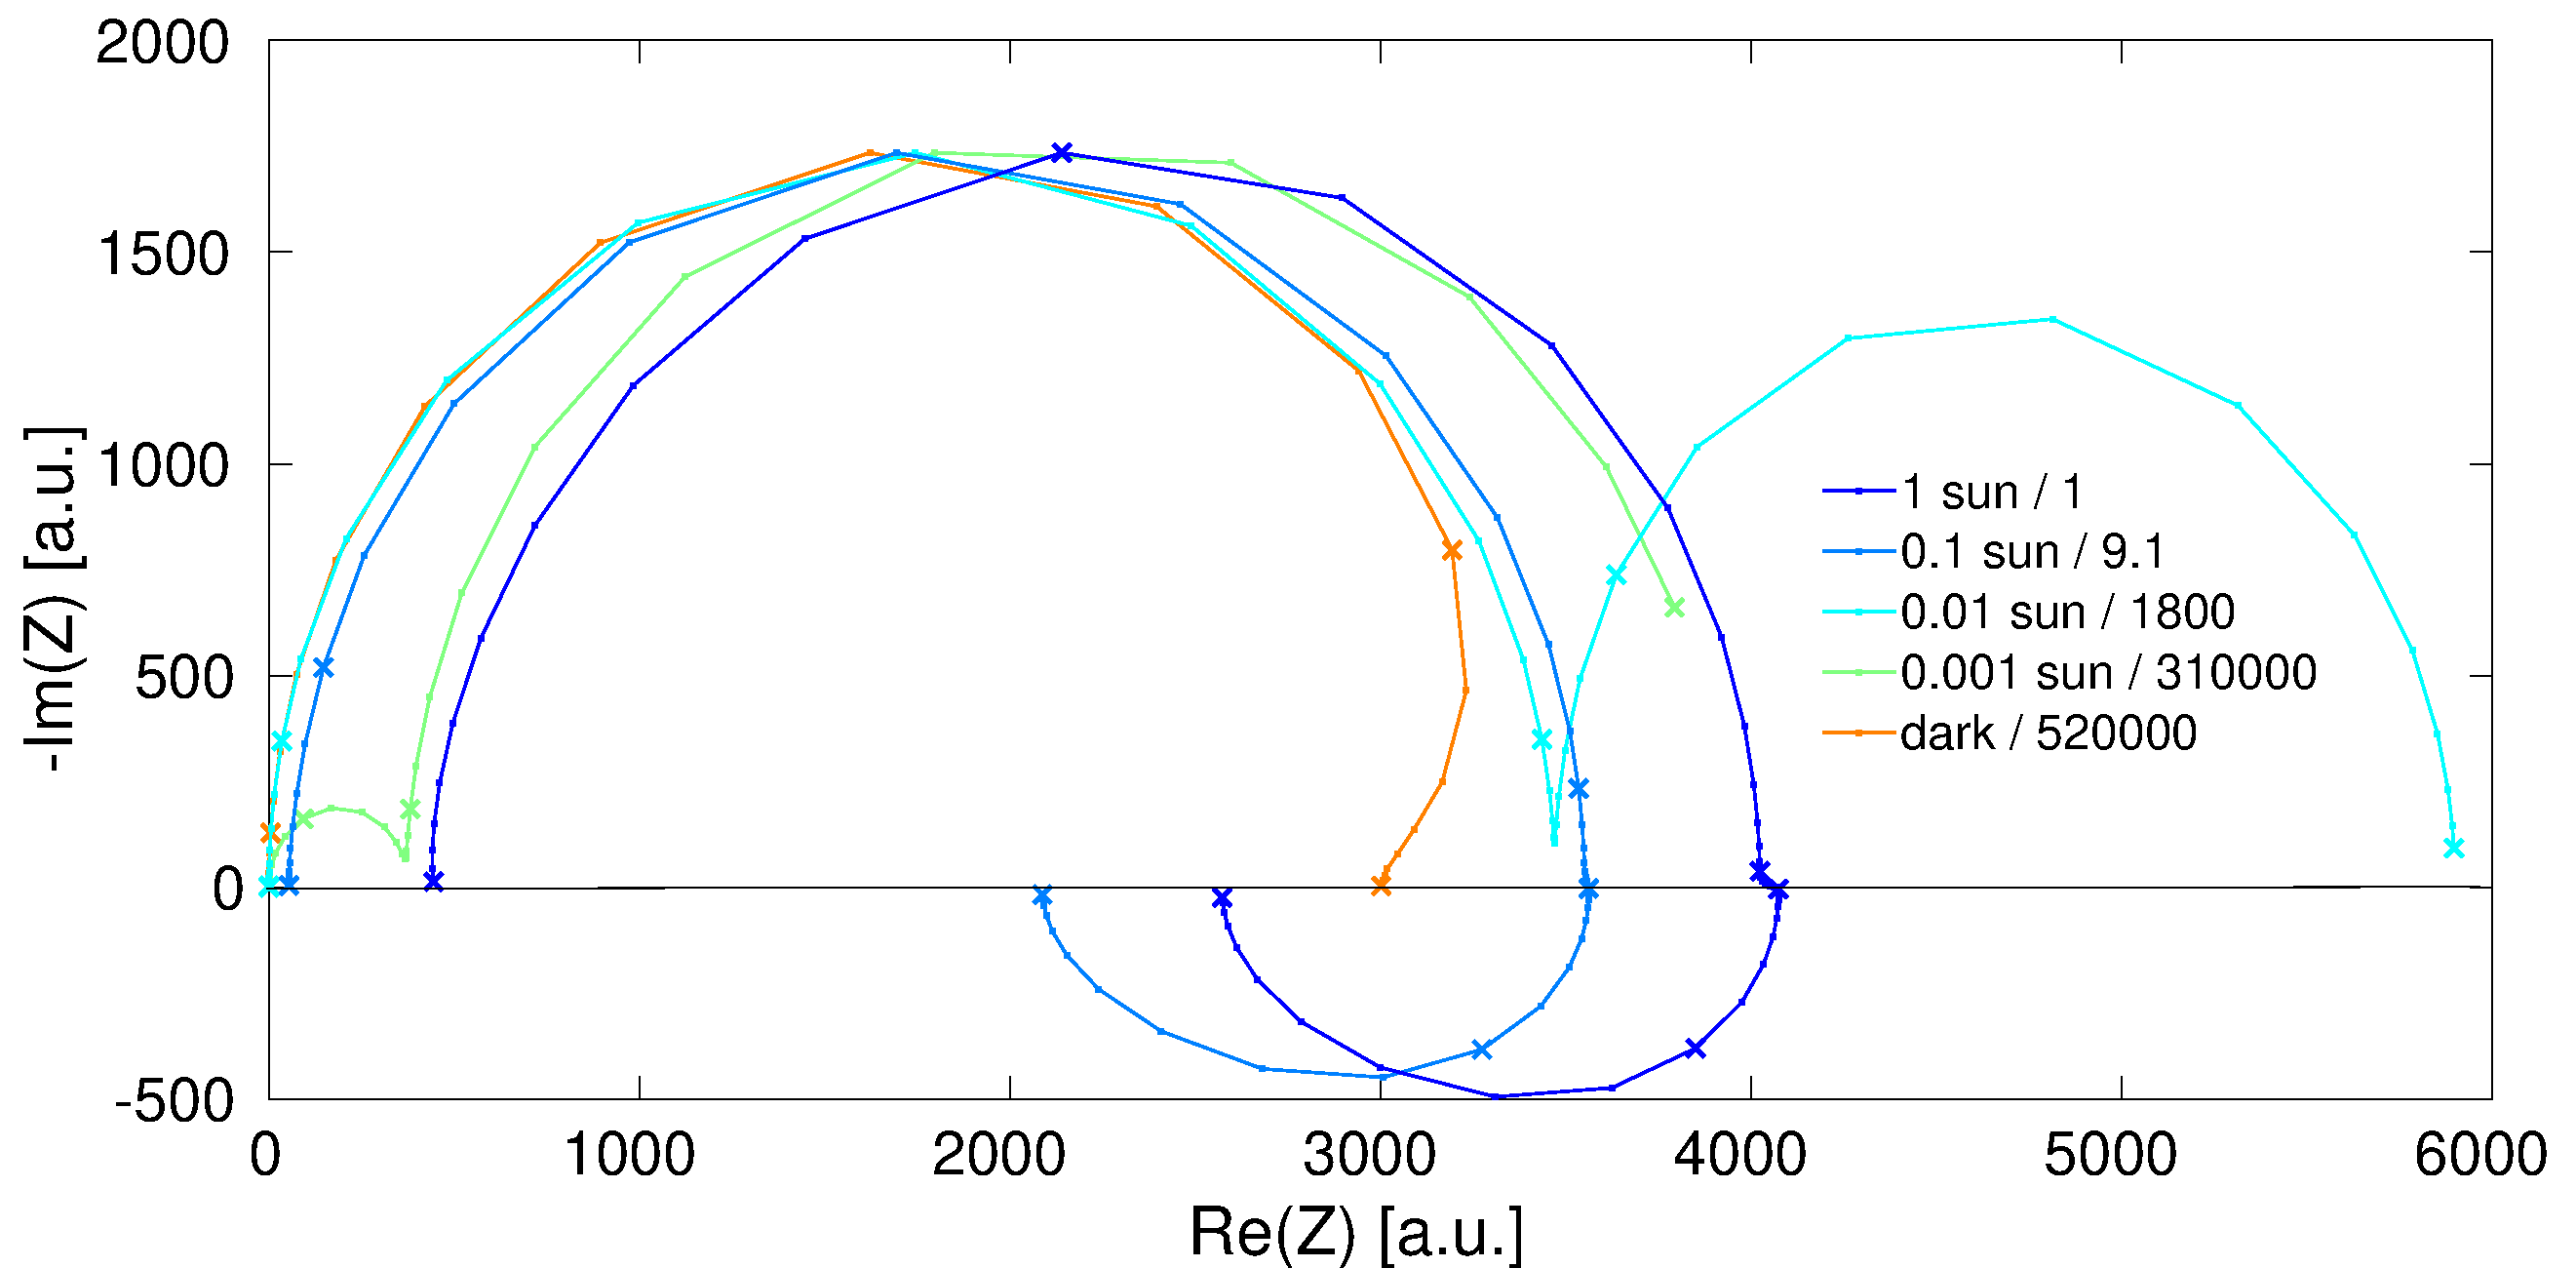
\includegraphics[width=1\textwidth]{heterojunction/ISwave_oc_nyquist_norm.png}
				\subcaption{Illuminated, open circuit, Nyquist}\label{fig:impedance_heterojunction-oc-nyquist}
			\end{subfigure}
			\qquad
			\begin{subfigure}[t]{0.51\textwidth}
				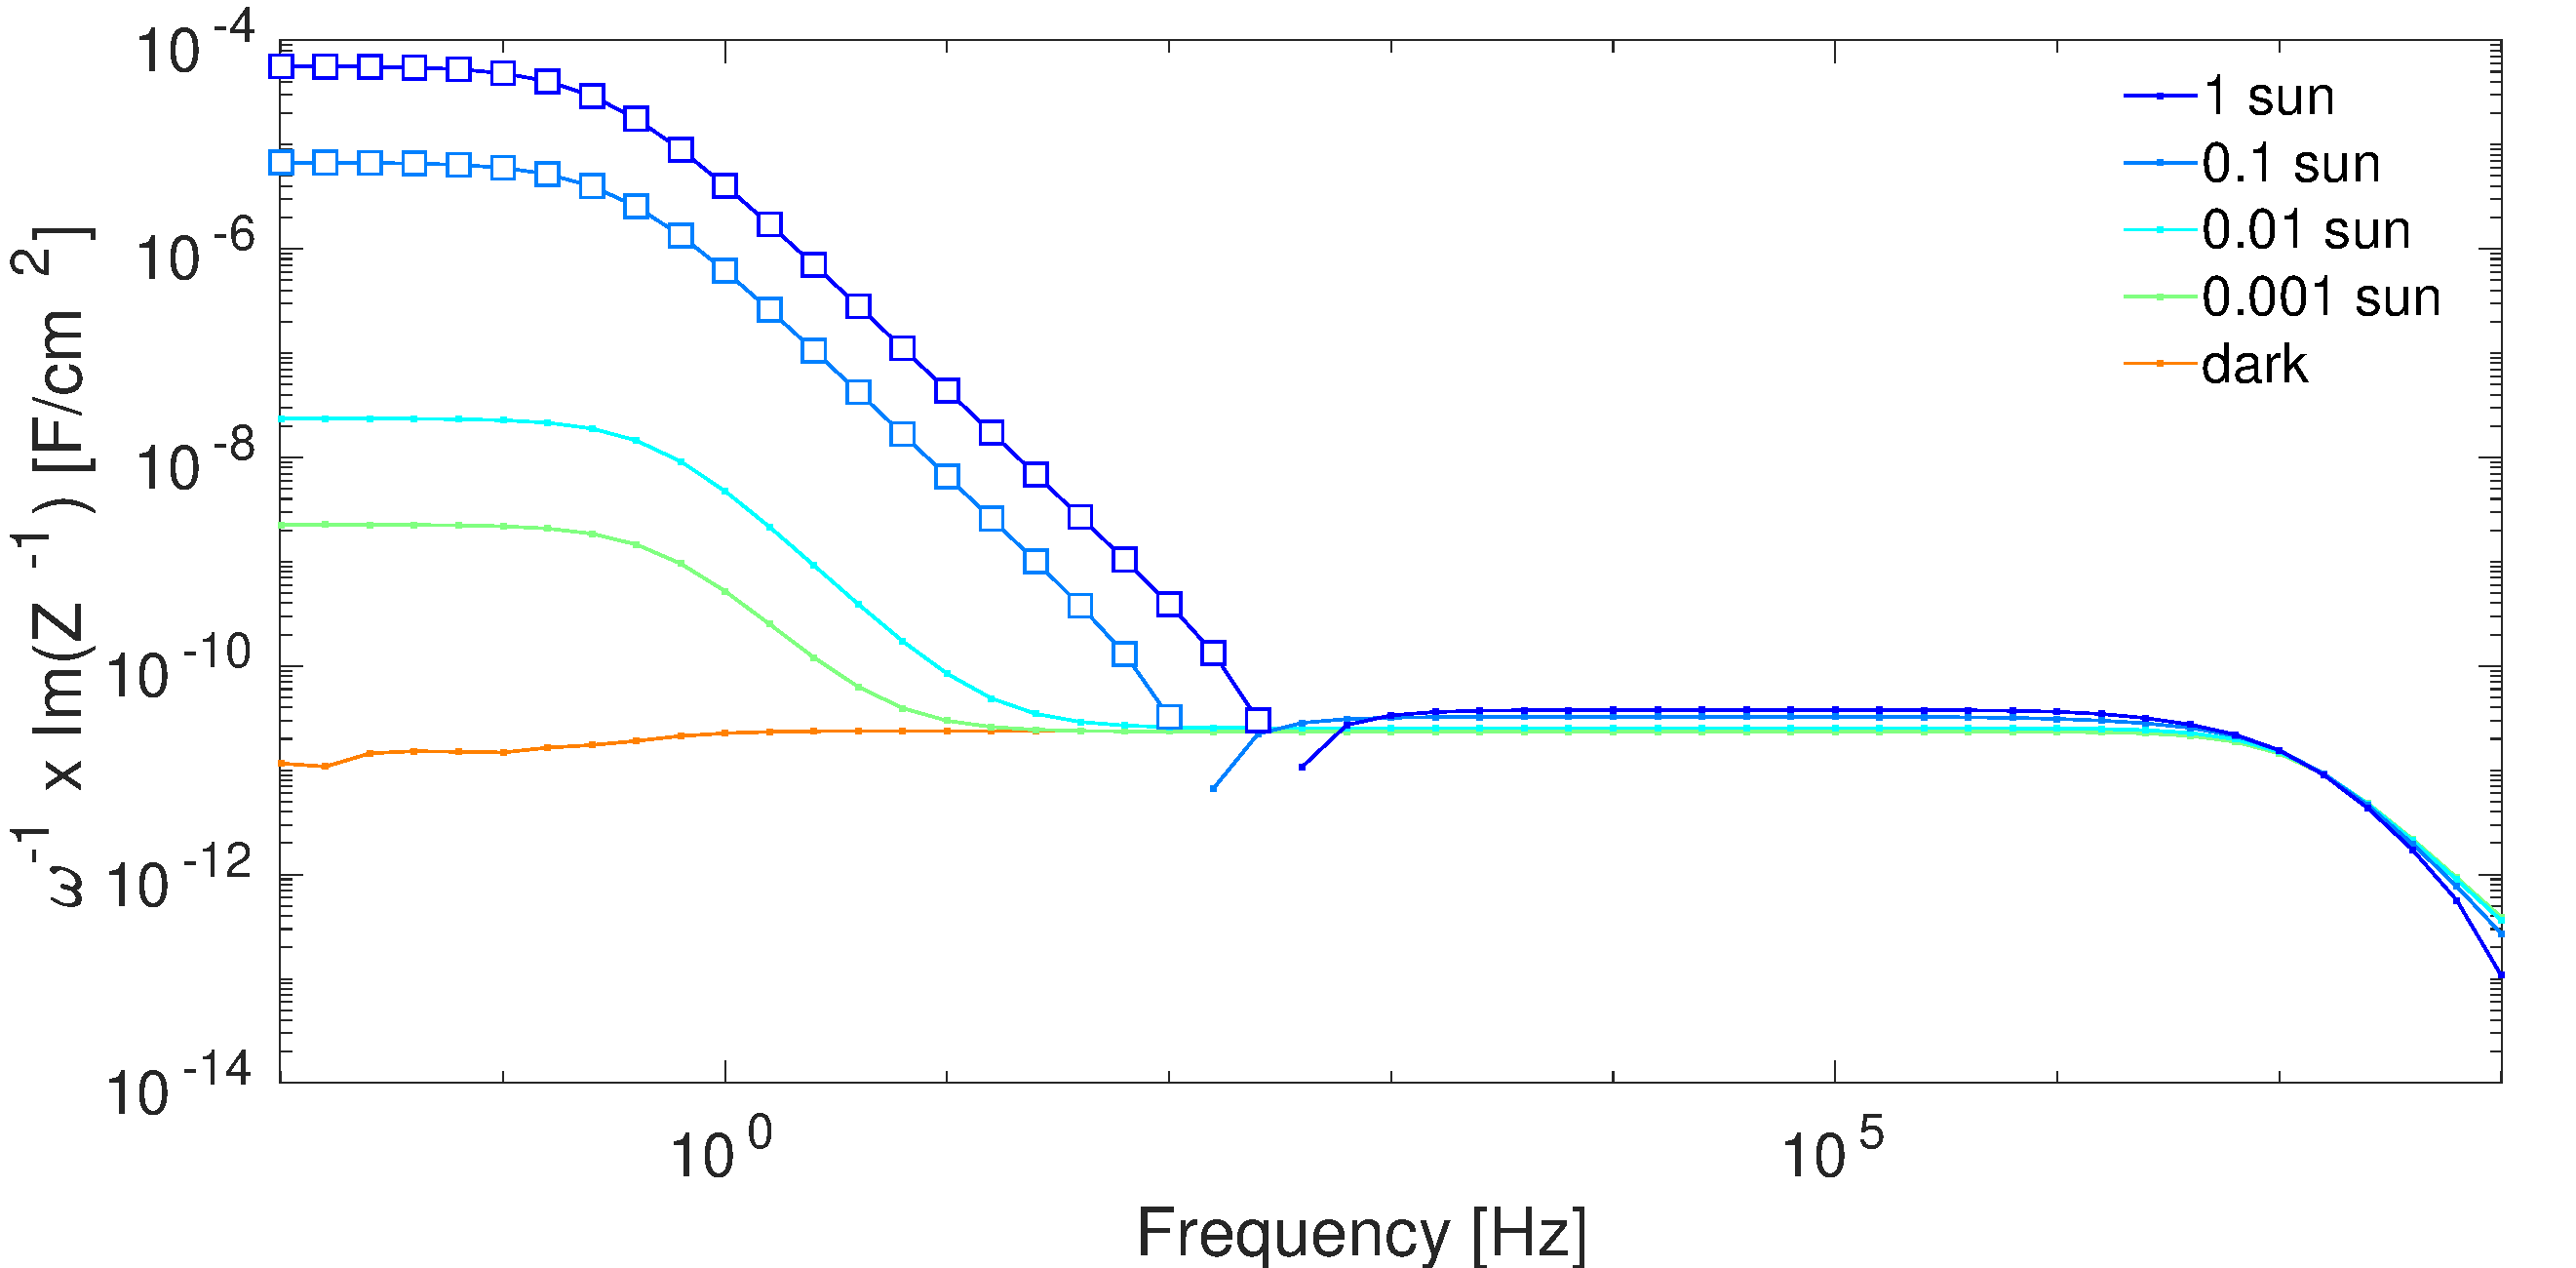
\includegraphics[width=1\textwidth]{heterojunction/ISwave_oc_cap.png}
				\subcaption{Illuminated, open circuit, apparent capacitance}\label{fig:impedance_heterojunction-oc-cap}
			\end{subfigure}
			\bigskip
			
			\begin{subfigure}[t]{0.51\textwidth}
				\includegraphics[width=1\textwidth]{heterojunction/ISwave_Vapp_nyquist_norm.png}
				\subcaption{Dark, applied voltage, Nyquist}\label{fig:impedance_heterojunction-vapp-nyquist}
			\end{subfigure}
						\qquad
			\begin{subfigure}[t]{0.51\textwidth}
				\includegraphics[width=1\textwidth]{heterojunction/ISwave_Vapp_cap.png}
				\subcaption{Dark, applied voltage, apparent capacitance}\label{fig:impedance_heterojunction-vapp-cap}
			\end{subfigure}
			\mycaption[Preliminary simulations of impedance on heterojunction model.]{The filled symbols indicate positive capacitance values, the hollow symbols represents negative capacitance which was changed in sign in order to be plotted on the same axis.}\label{fig:impedance_heterojunction}
		}
	}
\end{figure}


\paragraph{Heterojunction}
The simulations shown here are all based on a p-i-n homojunction model, so a proper injection barrier could not actually be simulated and the negative capacitance has been obtained playing with extreme values of other parameters as aforementioned.
An attempt of adapting the impedance scripts to the most recent heterojunction version of Driftfusion confirmed the presence of negative capacitance due to injection barrier modulation by ionic charge, as shown in \cref{impedance_heterojunction}.
Further work is needed for completely adapting the impedance scripts to the upstream heterojunction core code.






\paragraph{ElectroAbsorbance a.k.a. Stark spectroscopy}


\paragraph{Other similar techniques}
Using some modules already implemented for impedance spectroscopy simulation, it should be easy to implement also other characterization techniques like Intensity-Modulated Photovoltage/Photocurrent Spectroscopy (IMVS, IMPS) \cite{Pockett2015,Guillen2014} and Mott-Schottky capacitance analysis \cite{Almora2016}.



